\documentclass{article}
\usepackage[utf8]{inputenc}
\usepackage[T1]{fontenc}
\usepackage{graphicx}
\usepackage{algorithm}
\usepackage{algpseudocode}

\usepackage{listings}
\usepackage{xcolor}
\usepackage[margin=2cm]{geometry}
\usepackage{float}

\usepackage{amssymb} %Ajoute des symboles mathématiques comme R, Z, forall, exists, etc....
\usepackage{amsmath}
\usepackage{amsthm}


\lstdefinestyle{monstyle}{
    backgroundcolor=\color{white},
    commentstyle=\color{gray},
    keywordstyle=\color{blue},
    numberstyle=\tiny\color{gray},
    basicstyle=\ttfamily\small,
    breaklines=true,
    numbers=left,
    numbersep=5pt,
    frame=single,
}
\lstset{style=monstyle}

\usepackage{soul} % IMPORTANT : POUR SURLIGNER AVEC \hl en fin de ligne 
\usepackage{xcolor}

\title{\sethlcolor{purple!30}\hl{\textbf{Rapport de TD7: Initiation à l'algorithmique}}}
\author{Derrez Lorenzo}

\begin{document}
\maketitle

\section*{\hl{Exercice 1:}}

\subsection*{Question 1;}
\begin{itemize}
    \item Première séquence: $(0,1,3)$ 
    \item Deuxième séquence: $(0,1,7)$
    \subitem On retrouve bien 1,2, et 1.
\end{itemize}

\subsection*{Question 2;}

Soit B un mot de longueur $|B| = n$.

Pour chaque indice on a 2 choix:
\begin{itemize}
    \item on le garde;
    \item on ne le garde pas.
\end{itemize}

Puis on fait cela pour les n éléments $ \implies  2\times \ldots \times 2 \text{ (n fois)}  = 2^n $

\subsection*{Question 3;}

Par rapport à l'exemple 1; 
\begin{itemize}
    \item $ maxLG(B, C) = 5 $
    \item un plus long sous-mot commun de B et C est: $ 1 1 3 2 2 $
\end{itemize}

\subsection*{Question 4;}

On définit la caractérisation récursive suivante:

A est un sous-mot de B si:
\begin{itemize}
    \item Cas 1: A est vide;
    \item Cas 2: ou A est un sous-mot de $ B[1:|B|]$;
    \item Cas 3: ou $ A[0] == B[0] $ et $ A[1:|A|] $ est un sous-mot de $ B[1:|B|]$
\end{itemize}

\subsection*{Question 5;}

\begin{lstlisting}[label=python, caption={\textit{is\_sous-mot}}]
def is_sous-mot(A : Array[int], B: Array[int]) -> bool:
    i = 0 # position dans A
    j = 0 # position dans C
    while(i<len(A)) and (j<len(C)):
        if A[i]==C[j]:
            i += 1
        j += 1
    return len(A)==i
\end{lstlisting}

Evaluation des complexités:
\begin{itemize}
    \item En espace: Manipulation de variables entières uniquement $ \implies  \theta(n) $
    \item En temps: On avance de 1 à chaque itération $ \implies $ au maximum $ |C| $ itérations $ \implies  \theta(n) $
\end{itemize}

\subsection*{Question 6;}

\begin{lstlisting}[label=python, caption={\textit{tousSousmots}}]
def tousSousmots(B: Array[int])-> List(Array[int]):
    L = [[]]
    for x in B:
        n = len(L)
        for i in range(n):
            nouveau = L[i] + i
            L.append(nouveau)
    return L
\end{lstlisting}

Evaluation des complexités:
\begin{itemize}
    \item En espace: On crée L et on stock toutes les entrées en fonction de leur taille n. $ \implies \theta(n2^n) $
    \item En temps: de même, on copie tous les éléments de L[i]. Le coùt dépend donc de la longueur de ce sous-mot $ \implies \theta(n2^n) $
\end{itemize}

\subsection*{Question 7;}

\begin{lstlisting}[label=python, caption={\textit{maxLG}}]
def maxLG(B : Array[int], C: Array[int]) -> int:
    L = tousSousmots(B)
    current_max = 0
    for x in L:
        t = len(x)
        if t > current_max and is_sous-mot(x, C):
            current_max = t
    return current_max
\end{lstlisting}

\begin{itemize}
    \item Complexité en espace: $ \theta(n2^n) $ en lien avec la fonction \textit{tousSousmots}.
    \item Complexité en temps: $ \theta(n2^n) $ pour B et $\theta(m2^n) $ pour C $ \implies \theta((n+m)2^n) $
\end{itemize}

\subsection*{Question 8;}

On obtient, en lien avec la définiton de l'énoncé, les résultats suivants:
\begin{itemize}
    \item $ f(7,8) = 5 $
    \item $ f(0,8) = 0 $ 
    \item $ f(5,5) = 3 $ 
    \item $ f(5,4) = 3 $ 
    \item $ f(4,5) = 3 $
    \item $ f(4,4) = 2 $
    \item $ f(5,3) = 3 $
\end{itemize}

\subsection*{Question 9;}

\[
\forall i \in [0,|B|] \quad \forall j \in [0,|C|], f(i,j) = 
\begin{cases}
    0 \qquad \text{ si i = 0 ou j = 0}
    \\
    1 + f(i-1,j-1) \qquad \text{ si B[i-1] = C[j-1]}
    \\
    \max(f(i-1,j), f(i,j-1)) \qquad \text{ sinon}
\end{cases}
\]

\subsection*{Question 10;}

\begin{lstlisting}[label=python, caption={\textit{maxLG}}]
def maxLG(B: Array[int], C:Array[int]) -> int:
    i = len(B)
    j = len(C)
    if (i==0) or (j==0):
        return 0
    if B[i-1] == C[j-1]:
        return 1 + maxLG(B[:i-1], C[:j-1])
    return max(maxLG(B[:i-1], C[:j]), maxLG(B[:i], C[:j-1]))
\end{lstlisting}

\subsection*{Question 11;}

Evaluation de la complexité pour l'algorithme de la question 10.
\\
Dans le pire des cas:
\begin{itemize}
    \item $ n = |B|, m = |C| $
    \item $ \#f(n,m) = \theta(1) + \#f(n-1,m) + \#f(n,m-1) $
\end{itemize}
Entres autres, en dessinant l'arbre des appels:

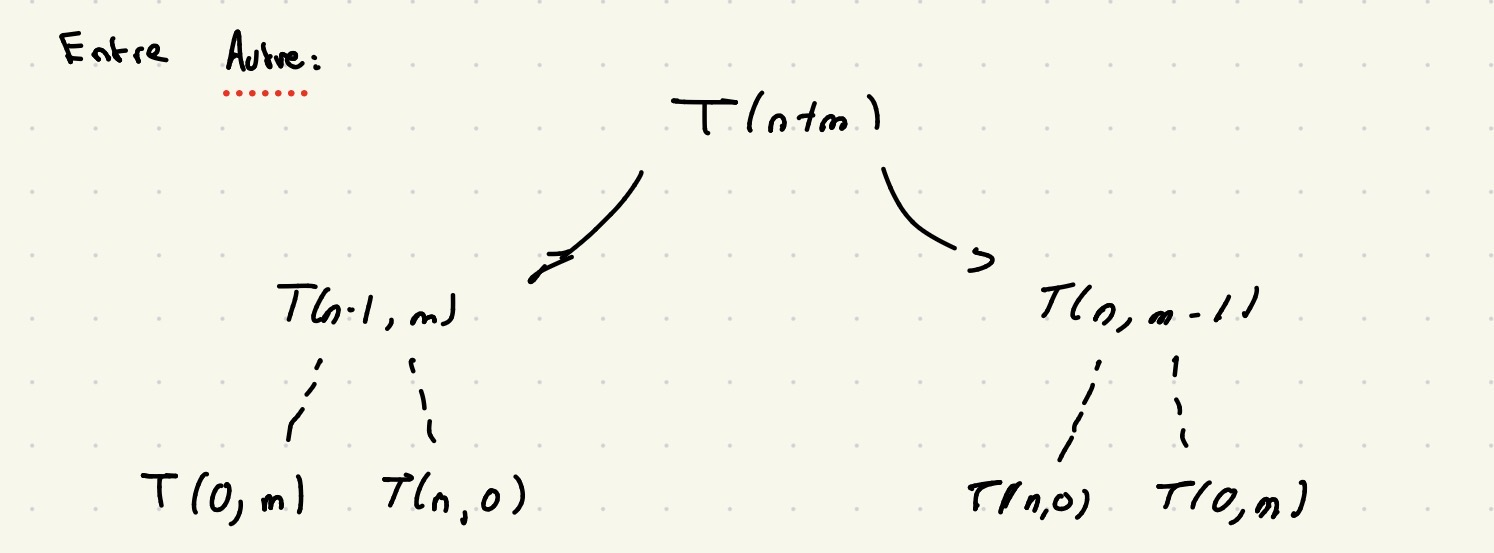
\includegraphics[width=0.60\textwidth]{arbre_TD7.jpeg}

Durant chaque appel;
\begin{itemize}
    \item peut produire au maximum 2 appels;
    \item la somme des longueurs n+m diminue de 1 à chaque descente dans l'arbre;
    \item la profondeur est au maximum de n+m
\end{itemize}

C'est donc une somme géométrique de raison 2: 

\[
    \displaystyle\sum_{k=0}^{n+m} 2^k = 2^{n+m+1}-1
\]

Par conséquent:
\[
    \text{Complexité en temps:} \implies O(2^{n+m})
\]

Pour la comlexité en espace:
\begin{itemize}
    \item on s'intéresse ici au maximum sur la pile d'appel;
    \item $\implies O(n+m)$
\end{itemize}

\subsection*{Question 12;}
Malgré l'amélioration en (Q10), on peut obtenir une situation où l'on calcul plusieurs fois un même calcul.
\\
Pour cela: programmation dynamique.

\begin{lstlisting}[label=python, caption={\textit{maxLG} programmation dynamique}]
def maxLG(B: Array[int], C: Array[int], memo: Array[int]) ->:
    i = len(B)
    j = len(C)
    if (i==0) or (j==0):
        return 0
    if (i,j) in memo:
        return memo[(i,j)]
    if B[i-1] == C[j-1]:
        resultat = 1 + maxLG(B[:i-1], C[:j-1], memo)
    resultat = max(maxLG(B[:i-1], C, memo), maxLG(B, C[:j-1], memo))
    memo[(i,j)] = resultat
    return memo[(i,j)]
\end{lstlisting}

Evaluation de la complexité:
\begin{itemize}
    \item $ n = |B|; m = |C| $
    \item En temps: $O(nm)$
    \item En espace: $O(nm)$
\end{itemize}

\subsection*{Question 13;}
A est un sous-mot maximal de B et C si:
\begin{itemize}
    \item $|A|$ est nul et $|B| \text{ ou } |C|$ est nul;
    \item B[|B|-1] = C[|C|-1] = A[|A|-1] et A[0:|A|-1] est un sous-mot maximal de B[0:|B|-1] et C[0:|C|-1]
    \item B[|B|-1] $!=$ C[|C|-1] et: 
    \subitem Si $f(|B|-1, |C|) > f(|B|, |C|-1)$ alors A est un sous-mot maximal de B[0; |B|-1] et C
    \subitem Sinon : A est un sous-mot maximal de B et C[0; |C|-1]
\end{itemize}

\subsection*{Question 15;}

\begin{lstlisting}[label=python, caption={\textit{SousmotMaximal}}]
def SousmotMaximal(B: Array[int], C: Array[int], memo: Array[int]) -> A:List[Array[int]]:
    i = len(B)
    j = len(C) 
    A = []

    while i > 0 and j > 0: 
        if B[i-1] == C[j-1]:
            A.append(B[i-1])
            i-=1
            j-=1
        elif memo[i-1][j] > memo[i][j-1]:
            i-=1
        else
            j-=1
    A.reverse()
    return A
\end{lstlisting}

\subsection*{Question 16;}

Evaluation de la complexité de l'algorithme de la question $(Q15)$.

\begin{itemize}
    \item En espace: $O(nm)$
    \item En temps: $O(nm)$
\end{itemize}

\section*{\hl{\textbf{Exercice 2:}}}

\subsection*{Question 1;}
-- Ensemble des combinaisons de 10 et $[2, 3, 5]$:
\[
    [2, 2, 0]; [0,0,2]; [5, 0, 0]; [1, 1, 1]
\]

\subsection*{Question 2;}


\end{document}